
% v2-acmsmall-sample.tex, dated March 6 2012
% This is a sample file for ACM small trim journals
%
% Compilation using 'acmsmall.cls' - version 1.3 (March 2012), Aptara Inc.
% (c) 2010 Association for Computing Machinery (ACM)
%
% Questions/Suggestions/Feedback should be addressed to => "acmtexsupport@aptaracorp.com".
% Users can also go through the FAQs available on the journal's submission webpage.
%
% Steps to compile: latex, bibtex, latex latex
%
% For tracking purposes => this is v1.3 - March 2012
\documentclass[prodmode,acmtecs]{acmsmall} % Aptara syntax
\usepackage[spanish,polish]{babel}
\usepackage[T1]{fontenc}
\usepackage{fancyvrb}
\usepackage{graphicx,hyperref}
\newcommand\cutout[1]{}


\usepackage[table]{xcolor}
\usepackage[utf8]{inputenc}
\usepackage[parfill]{parskip}
\usepackage{tabulary}
\PassOptionsToPackage{hyphens}{url}
\usepackage{hyperref}    
\usepackage[capitalize]{cleveref}


% Metadata Information
% !!! TODO: SET THESE VALUES !!!
\acmVolume{0}
\acmNumber{0}
\acmArticle{CFP}
\acmYear{0}
\acmMonth{0}

\newcounter{colstart}
\setcounter{page}{4}

\RecustomVerbatimCommand{\VerbatimInput}{VerbatimInput}%
{
%fontsize=\footnotesize,
fontfamily=\rmdefault
}


\newcommand{\UnderscoreCommands}{%\do\verbatiminput%
\do\citeNP \do\citeA \do\citeANP \do\citeN \do\shortcite%
\do\shortciteNP \do\shortciteA \do\shortciteANP \do\shortciteN%
\do\citeyear \do\citeyearNP%
}

\usepackage[strings]{underscore}



% Document starts
\begin{document}


\setcounter{colstart}{\thepage}

\acmArticle{CFP}
\title{{\huge\sc SIGLOG Monthly 256}

 December 2024}\author{ELLI ANASTASIADI\affil{Aalborg University, SE}\vspace*{-2.6cm}\begin{flushright}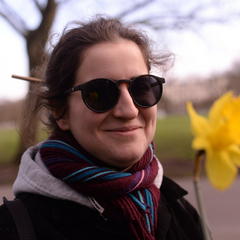
\includegraphics[width=30mm]{elli_anastasiadi.png}\end{flushright}}\begin{abstract}December 2024 edition of SIGLOG Monthly, featuring deadlines, calls and community announcements.
\end{abstract}


\maketitlee

\href{https://lics.siglog.org/newsletters/}{Past Issues}
 - 
\href{https://lics.siglog.org/newsletters/inst.html}{How to submit an announcement}
\section{Table of Contents}\begin{itemize}\item DEADLINES (\cref{deadlines}) 
 
\item SIGLOG MATTERS 
 
\begin{itemize}\item ANNOUNCEMENT (\cref{ANNOUNCEMENT})
\end{itemize} 
\item CALLS 
 
\begin{itemize}\item DisCoTec 2025 (CALL FOR PAPERS) (\cref{DisCoTec2025})
\item SPIN 2015 (CALL FOR PAPERS) (\cref{SPIN2015})
\item ACT 2025 (CALL FOR PAPERS) (\cref{ACT2025})
\item ECOOP 2025 WORKSHOPS (CALL FOR WORKSHOPS) (\cref{ECOOP2025WORKSHOPS})
\item DisCoTec 2025 (CALL FOR WORKSHOPS/TUTORIALS ) (\cref{DisCoTec2025})
\item SALOMA PRIZE (CALL FOR NOMINATIONS) (\cref{SALOMAPRIZE})
\end{itemize} 
\item JOB ANNOUNCEMENTS 
 
\begin{itemize}\item Senior Computer Science Professorship (\cref{SeniorComputerScienceProfessorship})
\end{itemize} 
\end{itemize}\section{Deadlines}\label{deadlines}\rowcolors{1}{white}{gray!25}\begin{tabulary}{\linewidth}{LL}SCD 2025 WORKSHOPS:  & Dec 12, 2024 (Workshop proposal) \\
LICS 2025:  & Jan 16, 2025 (Abstract), Jan 23, 2025 (Full Papers) \\
ECOOP 2025 WORKSHOPS:  & Jan 24, 2025 (Workshop proposals) \\
CiE 2025:  & Jan 26, 2025 (Abstract), Feb 02, 2025 (Full paper) \\
CAV 2025:  & Jan 31, 2025 (Full paper) \\
DisCoTec 2025:  & Jan 31, 2025 (Abstract), Feb 07, 2025 (Paper), Feb 10, 2025 (Workshop proposals) \\
FSCD 2025:  & Feb 10, 2025 (Abstract), Feb 17, 2025 (Full paper) \\
SPIN 2015:  & Feb 13, 2025 (Paper Submission), Feb 27, 2025 (Artifact Submission (Tool Papers)) \\
ACT 2025:  & Feb 26, 2025 (Abstract), Mar 03, 2025 (Paper) \\
SALOMA PRIZE:  & Feb 28, 2025 (Nomination deadline) \\
DEON 2025:  & Mar 01, 2025 (Abstract deadline), Mar 08, 2025 (Paper deadline) \\
Senior Computer Science Professorship:  & Mar 10, 2025 (Application deadline) \\
\end{tabulary}
\section{ANNOUNCEMENT}\label{ANNOUNCEMENT}Appeal to support SIGLOG, the LICS sponsor 

\begin{itemize}\item  Dear LICS colleagues, 
 
\item  This message addresses an important and timely subject concerning the sustainability of SIGLOG within ACM. 
 
\item  As some of you may already know, in 2022, ACM made the decision to increase the management fee (overhead) for its Special Interest Groups (SIGs), a fee that had remained steady for years. For smaller SIGs like ours, the minimum overhead increased from USD 10,000 to USD 25,000 annually. This change has significantly impacted SIGLOG's finances, and if we cannot find a way to pay the fee, we will be obliged to either merge SIGLOG with another SIG (the best choice, probably, would be SIGPLAN) or de-charter it altogether.  
 
\item  We requested additional time from ACM to explore ways of securing the financial foundation necessary to keep SIGLOG independent. We explained that our plan includes to seek increased industry sponsorship, grow our membership, and conduct fundraising activities at LICS and other events. ACM responded positively, SIGLOG now has until July 31, 2025, to develop a concrete, viable financial plan. 
 
\item  As a first step, we would like to ask you for support. This is not only a financial matter: to ensure our strength as a committed SIG, we need to increase our membership numbers. While the LICS community comprises around 2,600 people, SIGLOG currently has only about 200 members. We strongly encourage all LICS members to join SIGLOG. The membership fee is very affordable -- just 25 USD, a rate that has remained unchanged since the start of SIGLOG. We plan to maintain this rate, at least for students and early-career researchers, to support inclusivity. 
 
\item  Another goal is to promote industry sponsorship. Many in our community have strong connections with industry partners, and securing initial sponsorship would provide vital support as we work toward more stable, long-term financial solutions. If you have connections who might be interested in supporting SIGLOG, now is the time to reach out and explore potential sponsorship opportunities. 
 
\item  Finally, we invite your engagement, ideas, and shared experiences to help us build a sustainable future for SIGLOG. Your support is essential in ensuring that SIGLOG continues to exist as an independent entity dedicated to Logic. 
 
\item  Thank you very much for your time and consideration.  
 
\item  P.s. The SIGLOG web page is here: \href{https://siglog.org/}{https://siglog.org/}, and the instructions to join SIGLOG are here:  \href{https://siglog.org/membership/}{https://siglog.org/membership/}. Note that you don't need to have a separate ACM membership in order to subscribe to SIGLOG. 
 
\item  Best regards, Catuscia Palamidessi SIGLOG's chair, Also on behalf of the SIGLOG EC.  
 
\end{itemize}\section{DisCoTec 2025: 20th International Federated Conference on Distributed Computing Techniques}\label{DisCoTec2025}  Lille, France, 16-20 June 2025\\ 
  \href{https://www.discotec.org/2025}{https://www.discotec.org/2025}\\ 
CALL FOR PAPERS 

\begin{itemize}\item  DisCoTec 2025 is one of the major events sponsored by the International Federation for Information Processing (IFIP) and the European Association for Programming Languages and Systems (EAPLS). It gathers conferences and satellite events that cover a broad spectrum of distributed computing subjects — from theoretical foundations and formal description techniques, testing and verification methods, to language design and system implementation approaches. 
 
\item  MAIN CONFERENCES  
 
\begin{itemize}\item  COORDINATION (\href{https://www.discotec.org/2025/coordination}{https://www.discotec.org/2025/coordination}): 27rd International Conference on Coordination Models and Languages.  PC Chairs: Cinzia Di Giusto (Université Côte d’Azur, FR) and António Ravara (NOVA School of Science and Technology, PT)
\item  DAIS (\href{https://www.discotec.org/2025/dais}{https://www.discotec.org/2025/dais}): 25st International Conference on Distributed Applications and Interoperable Systems. PC Chairs: Daniel Balouek (INRIA, FR) and Ibéria Medeiros (University of Lisbon, PT)
\item  FORTE (\href{https://www.discotec.org/2025/forte}{https://www.discotec.org/2025/forte}): 45st International Conference on Formal Techniques for Distributed Objects, Components and Systems. PC Chairs: Carla Ferreira (NOVA University of Lisbon, PT) and Claudio A. Mezzina (University of Urbino, IT)
\end{itemize} 
\item  DisCoTec 2025 is organised by Inria Lille and the University of Lille. It will be hosted by Polytech Lille. 
 
\item  NEW: ACCOMODATIONS FOR PARENTS OF YOUNG CHILDREN 
 
  Subject to budget availability, we are planning to make special logistical arrangements for conference participants travelling with young children (and potentially accompanying persons). We invite interested persons to contact the General Chair (simon.bliudze@inria.fr), as soon as possible to discuss the arrangements that might be applicable. 
 
\item  KEYNOTE SPEAKERS  
 
\begin{itemize}\item  Alysson Bessani (Universidade de Lisboa, Portugal)
\item  Hélène Coullon (IMT Atlantique, France)
\item  Omar Inverso (GSSI, Italy)
\item  Burcu Ozkan (TU Delft, The Netherlands)
\end{itemize} 
\item  IMPORTANT DATES (for all main conferences).  
 
\rowcolors{1}{white}{gray!25}\begin{tabulary}{\linewidth}{LL}Abstract submission:  & Jan 31, 2025 \\
Paper submission:  & Feb 07, 2025 \\
Paper notification:  & Mar 28, 2025 \\
Camera-ready:  & 23 April 2025 (TBC) \\
DisCoTec conference:  & June 16-20, 2025 \\
\end{tabulary}
 
 All deadlines expire at 23:59 anywhere on earth. 
 
\item    See each conference site for topics of interest, paper categories, and submission instructions. 
 
\item  PROCEEDINGS  
 
  Main conference proceedings will be published as volumes in the Springer LNCS-IFIP series. The volumes will be open access from the IFIP digital library after a 3-year embargo. 
 
\item  Journal Special Issues 
 
  Selected papers accepted at the main conferences will be invited for submission to special issues in high-quality journals, such as: 
 
\begin{itemize}\item  Logical Methods in Computer Science
\item  Science of Computer Programming (Software Track).
\end{itemize} 
\end{itemize}\section{SPIN 2015: 31st International Symposium on Model Checking Software}\label{SPIN2015}  \href{https://spin-web.github.io/SPIN2025/}{https://spin-web.github.io/SPIN2025/}\\ 
  7 - 8 May 2025\\ 
  co-located with ETAPS 2025, Hamilton, Canada\\ 
CALL FOR PAPERS 

\begin{itemize}\item  OVERVIEW 
 
  The SPIN symposium aims at bringing together researchers and practitioners interested in automated tool-based techniques for the analysis of software as well as models of software, for the purpose of verification and validation. The symposium specifically focuses on concurrent software but does not exclude the analysis of sequential software. Submissions are solicited on theoretical results, novel algorithms, tool development, and empirical evaluation.  
 
\item  The SPIN symposium originated as a workshop focusing on explicit state model checking, specifically as related to the SPIN model checker. However, over the years it has evolved to a broadly-scoped symposium for software analysis using any automated techniques, including model checking, automated theorem proving, and symbolic execution. An overview of the previous SPIN symposia (and early workshops) can be found at: \href{https://spinroot.com/spin/Workshops/}{https://spinroot.com/spin/Workshops/}. 
 
\item  A full list of the topics of interest can be found at \href{https://spin-web.github.io/SPIN2025/cfp}{https://spin-web.github.io/SPIN2025/cfp} together with submission instructions and details.  
 
\item  IMPORTANT DATES:  
 
\rowcolors{1}{white}{gray!25}\begin{tabulary}{\linewidth}{LL}Paper Submission:  & Feb 13, 2025 \\
Artifact Submission (Tool Papers):  & Feb 27, 2025 \\
Paper/Artifact Notifications:  & Mar 24, 2025 \\
Artifact Submission (Other Papers):  & Mar 12, 2025 \\
Non-tool Paper Artifact Notification:  & May 01, 2025 \\
Symposium:  & May 7-8, 2025 \\
\end{tabulary}
 
\item  ARTIFACT EVALUATION: 
 
  SPIN 2025 will feature artifact evaluation, performed by an Artifact Evaluation Committee (AEC). The AEC evaluates artifacts based on documentation, availability, reproducibility of results, and tool reusability (if applicable). Artifact submission is mandatory for Full Tool Papers. While artifact submission is optional for papers in other categories, we highly encourage authors of papers involving tool development and empirical evaluation to submit an artifact for evaluation. Papers with an accompanying artifact may be awarded one or more badges from the EAPLS artifact badging scheme (\href{https://eapls.org/pages/artifact_badges/}{https://eapls.org/pages/artifact\_badges/}). More details can be found at: \href{https://spin-web.github.io/SPIN2025/artifacts}{https://spin-web.github.io/SPIN2025/artifacts} . 
 
\item  KEYNOTE SPEAKERS:   
 
\begin{itemize}\item  Alexandre Duret-Lutz (EPITA Research Laboratory (LRE))
\item  Orna Grumberg (Technion, Israel)
\end{itemize} 
\item  PC CHAIRS: 
 
\begin{itemize}\item  Gidon Ernst (Ludwig-Maximilians-Universität München)
\item  Kristin Yvonne Rozier (Iowa State University) 
\end{itemize} 
\item  This edition of SPIN will include artifact evaluation, cf. \href{https://spin-web.github.io/SPIN2025/artifacts}{https://spin-web.github.io/SPIN2025/artifacts}. We are now forming an Artifact Evaluation Committee headed by our artifact evaluation chairs: 
 
\begin{itemize}\item  Julie Cailler (University of Lorraine \& Inria, France)
\item  Nian-Ze Lee (LMU Munich / National Taiwan University)
\end{itemize} 
\item  If you have experience in artifact creation and evaluation or a passion for tools and empirical experiments, you are welcome to nominate yourself via an email to the AEC chairs. 
 
\end{itemize}\section{ACT 2025: APPLIED CATEGORY THEORY  }\label{ACT2025}  University of Florida on June 2-6, 2025\\ 
  \href{https://gataslab.org/act2025/act2025cfp}{https://gataslab.org/act2025/act2025cfp}\\ 
CALL FOR PAPERS 

\begin{itemize}\item  The Eighth International Conference on Applied Category Theory (\href{https://easychair.org/cfp/ACT2025}{https://easychair.org/cfp/ACT2025}) will take place at the University of Florida on June 2-6, 2025. The conference will be preceded by the Adjoint School on May 26-30, 2025. This conference follows previous events at Oxford (2024, 2019), University of Maryland (2023), Strathclyde (2022), Cambridge (2021), MIT (2020), and Leiden (2019).  
 
  Applied category theory is important to a growing community of researchers who study computer science, logic, engineering, physics, biology, chemistry, social science, systems, linguistics and other subjects using category-theoretic tools. The background and experience of our members is as varied as the systems being studied. The goal of the Applied Category Theory conference series is to bring researchers together, strengthen the applied category theory community, disseminate the latest results, and facilitate further development of the field. 
 
\item IMPORTANT DATES  
 
  All deadlines are AoE (Anywhere on Earth). 
 
\rowcolors{1}{white}{gray!25}\begin{tabulary}{\linewidth}{LL}Abstract submission:  & Feb 26, 2025 \\
Paper submission:  & Mar 03, 2025 \\
Notifiaction:  & Apr 07, 2025 \\
Final versions:  & May 19, 2025 \\
Conference:  & June 2-6, 2025 \\
\end{tabulary}
 
\item  SUBMISSIONS 
 
  The submission URL is: \href{https://easychair.org/conferences/?conf=act2025}{https://easychair.org/conferences/?conf=act2025} . We accept submissions in English of original research papers, talks about work accepted/submitted/published elsewhere, and demonstrations of relevant software. Accepted original research papers will be published in a proceedings volume. The conference will include an industry showcase event and community meeting. We particularly encourage people from underrepresented groups to submit their work and the organizers are committed to non-discrimination, equity, and inclusion. 
 
  Conference Papers should present original, high-quality work in the style of a computer science conference paper (up to 12 pages, not counting the bibliography; more detailed parts of proofs may be included in an appendix for the convenience of the reviewers). Such submissions should not be an abridged version of an existing journal article although pre-submission arXiv preprints are permitted. These submissions will be adjudicated for both a talk and publication in the conference proceedings. 
 
  Talk proposals not to be published in the proceedings, e.g. about work accepted/submitted/published elsewhere, should be submitted as abstracts, one or two pages long. Authors are encouraged to include links to any full versions of their papers, preprints or manuscripts. The purpose of the abstract is to provide a basis for determining the topics and quality of the anticipated presentation. 
 
  Software demonstration proposals should also be submitted as abstracts, one or two pages. The purpose of the abstract is to provide the program committee with enough information to assess the content of the demonstration. 
 
\item  The selected conference papers will be published in a volume of Proceedings. Authors are advised to use EPTCS style; files are available at style.eptcs.org. Reviewing will be single-blind, and we are not making public the reviews, reviewer names, the discussions nor the list of under-review submissions. This is the same as previous instances of ACT. In order to give our reviewers enough time to bid on submissions, we ask for a title and brief abstract of your submission by February 26. The full two-page pdf extended abstract submissions and up to 12 page proceedings submissions are both due by the submissions deadline of March 3 11:59pm AoE (Anywhere on Earth). 
 
\item  Please contact the Programme Committee Chairs for more information: Amar Hadzihasanovic (amar.hadzihasanovic@taltech.ee) and JS Lemay (js.lemay@mq.edu.au). 
 
  Programme Committee: See conference website for full list: \href{https://gataslab.org/act2025/act2025cfp}{https://gataslab.org/act2025/act2025cfp} 
 
\end{itemize}\section{ECOOP 2025 WORKSHOPS}\label{ECOOP2025WORKSHOPS}  Mon 30 June - Fri 4 July 2025 Bergen, Norway\\ 
  \href{https://2025.ecoop.org/track/ecoop-2025-workshops#Call-for-Workshops}{https://2025.ecoop.org/track/ecoop-2025-workshops\#Call-for-Workshops}\\ 
CALL FOR WORKSHOPS 

\begin{itemize}\item  Overview 
 
  ECOOP (the European Conference on Object-Oriented Programming) hosts a diverse offering of workshops bringing together academics, industrial researchers, and practitioners to exchange new ideas, problems, and experiences. Topics for workshops may include, but are not limited to, the theory, design, implementation, optimization, testing, and analysis of programs and programming languages. Workshops will run after the program of the main conference (Thu. 3 - Fri. 4 July 2025). The organizers will investigate the possibility of organizing the publication of a single-volume peer-reviewed post-proceedings if there is enough interest. Submission link: \href{https://framaforms.org/proposal-for-ecoop25-workshop-1729617158}{https://framaforms.org/proposal-for-ecoop25-workshop-1729617158} Please contact ECOOP'25 workshops chair, Clément Aubert (caubert@augusta.edu or clement.aubert@math.cnrs.fr), if you have any questions. 
 
\item  Timeline: 
 
  Workshop proposals will be reviewed on a rolling basis, with the last submission date being on January 24, 2025. 
 
Workshop proposals: Jan 24, 2025 
 
  Workshops must send notifications for accepted papers by June 21, 2025, which will be about one week before the early registration deadline. 
 
  The workshop’s website must be live within two weeks of notification of the workshop’s acceptance and include relevant information about the organizers and any call for contributions. 
 
\item  To submit a proposal for an ECOOP'25 workshop, please complete the online form linked above. After submitting, you will receive an automated email confirmation of your submission and, within at most four weeks (or shortly after the final submission deadline), a formal response notifying you if the workshop has been accepted for ECOOP'25. 
 
\end{itemize}\section{DisCoTec 2025: 20th International Federated Conference on Distributed Computing Techniques}\label{DisCoTec2025}  Lille, France, 16-20 June 2025\\ 
  \href{https://www.discotec.org/2025}{https://www.discotec.org/2025}\\ 
CALL FOR WORKSHOPS/TUTORIALS  

\begin{itemize}\item  SATELITE EVENTS 
 
\item  The DisCoTec 2025 organising committee invites proposals for satellite events to complement the three main conferences. The aim is to provide a vivid and open forum for discussions, presentations of preliminary research results and ongoing work, as well as presentations of research work to a focussed audience. The satellite events will be held in conjunction with the main events. Prospective satellite event chairs should contact the organisers and provide the following information: 
 
\begin{itemize}\item  the name and the preferred date of the proposed satellite event (June 16 or 20, 2025);
\item  a short description of the satellite event (up to 300 words);
\item  if applicable, a description of past editions of the satellite event, including dates, organizers, submission and acceptance counts, and attendance;
\item  the name and short CV of the organizer(s);
\item  the expected number of participants;
\item  for tutorials: the DisCoTec conference most related to the proposed tutorial (COORDINATION, DAIS, FORTE);
\item  for workshops: the publication plan (only invited speakers, no published proceedings, pre-/post-proceedings published with EPTCS/ENTCS/...).
\end{itemize} 
\item  IMPORTANT DATES:  
 
\rowcolors{1}{white}{gray!25}\begin{tabulary}{\linewidth}{LL}Workshop proposals submission:  & Feb 10, 2025 \\
Notification of accepted satellite events:  & Mar 01, 2025 \\
Paper submission deadline:  & Mid April, 2025 \\
Notification of accepted papers:  & Mid May, 2025 \\
Satellite events:  & June 16 or 20, 2025 \\
\end{tabulary}
 
\item  The submission and notification deadlines of the satellite events are at the discretion of the individual event chairs. However, the notification must be no later than the early registration deadline for DisCoTec 2025 (to be announced). 
 
\item  DisCoTec 2025 Satellite Events Chair 
 
\begin{itemize}\item  Larisa Safina (INRIA, FR), discotec-satellite@inria.fr
\end{itemize} 
\end{itemize}\section{SALOMA PRIZE }\label{SALOMAPRIZE}CALL FOR NOMINATIONS 

\begin{itemize}\item  The Salomaa Prize in Automata Theory, Formal Languages, and Related Topics is awarded annually at the conference DLT (Developments in Language Theory). It consists of the diploma and the prize of 2000 Euros donated by the University of Turku. The award is given to a distinguished researcher for their fundamental achievements in automata theory and related topics. The achievement might be a single article, a series of articles, or broader impact on the theory. The main criterion is the scientific excellence of the work. The Salomaa Prize 2025 will be awarded at DLT 2025 in Seoul, Korea. The deadline for nomination is February 28 2025. Nominations, which consist of a description of the nominee's work and rationale for the award, signed by at least two recognized researchers, should be sent by electronic mail to the chair of the selection committee: Jeffrey Shallit, University of Waterloo, shallit@uwaterloo.ca 
 
\item  For all further information, see the guidelines on the Salomaa Prize website: \href{https://math.utu.fi/salomaaprize/}{https://math.utu.fi/salomaaprize/} 
 
Nomination deadline: Feb 28, 2025 
 
\end{itemize}\section{Senior Computer Science Professorship: Oxford University}\label{SeniorComputerScienceProfessorship}JOB ANNOUNCEMENT 

\begin{itemize}\item  Oxford University’s Computer Science Department (together with St John's College at Oxford) is hiring a senior Professor in Computer Science. We are looking for somebody with a world-leading research reputation with broad academic leadership. For more information, see: \href{https://my.corehr.com/pls/uoxrecruit/erq_jobspec_details_form.jobspec?p_id=173846}{https://my.corehr.com/pls/uoxrecruit/erq\_jobspec\_details\_form.jobspec?p\_id=173846} 
 
Application deadline: Mar 10, 2025 
 
\end{itemize}


\bigskip Links: \href{http://siglog.org/}{SIGLOG website}, \href{https://lics.siglog.org}{LICS website}, \href{https://lics.siglog.org/newsletters/}{SIGLOG Monthly}\end{document}